\section{Packaging research artefacts with RO-Crate}
\label{ch5:packaging-research-artefacts-with-ro-crate}

An increasing number of researchers support reproducibility by including
pointers to and descriptions of datasets, software and methods in their
publications. However, scientific articles may be ambiguous, incomplete
and difficult to process by automated systems. In this paper we
introduce RO-Crate, an open, community-driven, and lightweight approach
to packaging research artefacts along with their metadata in a machine
readable manner. RO-Crate is based on schema.org annotations in JSON-LD,
aiming to establish best practices to formally describe metadata in an
accessible and practical way for their use in a wide variety of
situations.

An RO-Crate is a structured archive of all the items that contributed to
a research outcome, including their identifiers, provenance, relations
and annotations. As a general purpose packaging approach for data and
their metadata, RO-Crate is used across multiple areas, including
bioinformatics, digital humanities and regulatory sciences. By applying
``just enough'' Linked Data standards, RO-Crate simplifies the process
of making research outputs FAIR while also enhancing research
reproducibility.

\subsection{Introduction}\label{ch5:introduction}

The move towards Open Science has increased the need and demand for the
publication of artefacts of the research process
\cite{Sefton 2021a}. This is
particularly apparent in domains that rely on computational experiments;
for example, the publication of software, datasets and records of the
dependencies that such experiments rely on
\cite{Stodden 2016}.

It is often argued that the publication of these assets, and
specifically software
\cite{Lamprecht 2019}, workflows
\cite{Goble 2020} and data, should
follow the FAIR principles
\cite{Wilkinson 2016}; namely, that
they are Findable, Accessible, Interoperable and Reusable. These
principles are agnostic to the \emph{implementation} strategy needed to
comply with them. Hence, there has been an increasing amount of work in
the development of platforms and specifications that aim to fulfil these
goals \cite{Mons 2018}.

Important examples include data publication with rich metadata
(e.g.~Zenodo \cite{Dillen 2019a}),
domain-specific data deposition (e.g.~PDB
\cite{Berman 2007}) and following
practices for reproducible research software
\cite{Sandve 2013} (e.g.~use
of containers). While these platforms are useful, experience has shown
that it is important to put greater emphasis on the interconnection of
the multiple artefacts that make up the research process
\cite{Koesten 2021}.

The notion of \textbf{Research Objects}
\cite{Bechhofer 2013}
(RO) was introduced to address this connectivity, providing semantically
rich \emph{aggregations} of (potentially distributed) resources with a
layer of structure over a research study; this is then to be delivered
in a \emph{machine-readable format}.

A Research Object combines the ability to bundle multiple types of
artefacts together, such as spreadsheets, code, examples, and figures.
The RO is augmented with annotations and relationships that describe the
artefacts' \emph{context} (e.g.~a CSV being used by a script, a figure
being a result of a workflow).

This notion of ROs provides a compelling vision as an approach for
implementing FAIR data. However, existing Research Object
implementations require a large technology stack
\cite{Belhajjame 2015}, are
typically tailored to a particular platform and are also not easily
usable by end-users.

To address this gap, a new community came together
\cite{Ó Carragáin 2019a} to develop
\textbf{RO-Crate} --- an \emph{approach to package and aggregate
research artefacts with their metadata and relationships}. The aim of
this paper is to introduce RO-Crate and assess it as a strategy for
making multiple types of research artefacts FAIR. Specifically, the
contributions of this paper are as follows:

\begin{enumerate}
  \item An introduction to RO-Crate, its purpose and context.
  \item A guide to the RO-Crate community and tooling.
  \item Examples of RO-Crate usage, demonstrating its value as connective tissue for different artefacts from different communities.
\end{enumerate}

The rest of this article is organised as follows. We first describe
RO-Crate through its development methodology that formed the RO-Crate
concept, showing its foundations in Linked Data and emerging principles.
We then define RO-Crate technically, before we introduce the community
and tooling. We move to analyse RO-Crate with respect to usage in a
diverse set of domains. Finally, we present related work and conclude
with some remarks including RO-Crate highlights and future work. The
appendix to this article (section \vref{ch5:formaldefinition}) adds a formal definition of RO-Crate using First-Order logic.

\subsection{RO-Crate}\label{ch5:rocrate}

RO-Crate aims to provide an approach to packaging research artefacts
with their metadata that can be easily adopted. To illustrate this, let
us imagine a research paper reporting on the sequence analysis of
proteins obtained from an experiment on mice. The sequence output files,
sequence analysis code, resulting data and reports summarising
statistical measures are all important and inter-related research
artefacts, and consequently would ideally all be co-located in a
directory and accompanied with their corresponding metadata. In reality,
some of the artefacts (e.g.~data or software) will be recorded as
external reference to repositories that are not necessarily following
the FAIR principles. This conceptual directory, along with the
relationships between its constituent digital artefacts, is what the
RO-Crate model aims to represent, linking together all the elements of
an experiment that are required for the experiment's reproducibility and
reusability.

The question then arises as to how the directory with all this material
should be packaged in a manner that is accessible and usable by others.
This means programmatically and automatically accessible by machines and
human-readable. A de facto approach to sharing collections of resources
is through compressed archives (e.g.~a ZIP file). This solves the
problem of ``packaging'', but it does not guarantee downstream access to
all artefacts in a programmatic fashion, nor describe the role of each
file in that particular research. Both features, the ability to
automatically access and reason about an object, are crucial and lead to
the need for explicit metadata about the contents of the folder,
describing each and linking them together.

Examples of metadata descriptions across a wide range of
domains\footnote{\url{https://rdamsc.bath.ac.uk/scheme-index}} abound within the
literature, both in research data management
\cite{Amorim 2016,Farnel 2014,Kurowski 2021}
and within library and information
systems\footnote{\url{https://www.loc.gov/librarians/standards}} \cite{Mai Chan 1995,Žumer 2009}. However, many of these approaches require
knowledge of metadata schemas, particular annotation systems, or the
use of complex software stacks. Indeed, particularly within research,
these requirements have led to a lack of adoption and growing
frustration with current tooling and specifications
\cite{Neylon 2017,Volk 2014,Schriml 2020}.

RO-Crate seeks to address this complexity by:

\begin{enumerate}
  \item Being conceptually simple and easy to understand for developers.
  \item Providing strong, easy tooling for integration into community projects.
  \item Providing a strong and opinionated guide regarding current best practices.
  \item Adopting de-facto standards that are widely used on the Web.
\end{enumerate}

In the following sections we demonstrate how the RO-Crate specification
and ecosystem achieve these goals.

\subsubsection{Development Methodology}\label{ch5:methodology}

It is a good question as to what base level we assume for `conceptually
simple'. We take simplicity to apply at two levels: for the
\emph{developers} who produce the platforms and for the \emph{data
practitioners} and users of those platforms.

For our development methodology we followed the mantra of working
closely with a small group to really get a deep understanding of
requirements and ensure rapid feedback loops. We created a pool of early
adopter projects from a range of disciplines and groups, primarily
addressing developers of platforms. Thus the base level for simplicity
was \textbf{developer friendliness}.

We assumed a developer familiar with making Web applications with JSON
data (who would then learn how to make \emph{RO-Crate JSON-LD}), which
informed core design choices for our JSON-level documentation approach
and RO-Crate serialization (section \vref{ch5:implementation}). Our group of early
adopters, growing as the community evolved, drove the RO-Crate
requirements and provided feedback through our multiple communication
channels including bi-monthly meetings, which we describe in section \vref{ch5:community} along with the established norms.

Addressing the simplicity of understanding and engaging with RO-Crate by
data practitioners is through the platforms, for example with
interactive tools (section \vref{ch5:tooling}) like
Describo\footnote{\url{https://arkisto-platform.github.io/describo/}} \cite{La Rosa 2021d} and
Jupyter notebooks
\cite{Kluyver 2016}, and by
close discussions with domain scientists on how to appropriately capture
what they determine to be relevant metadata. This ultimately requires a
new type of awareness and learning material separate from developer
specifications, focusing on the simplicity of extensibility to serve the
user needs, along with user-driven development of new RO-Crate Profiles
specific for their needs (section \vref{ch5:inuse}).

\subsubsection{Conceptual Definition}\label{ch5:conceptual}

A key premise of RO-Crate is the existence of a wide variety of
resources on the Web that can help describe research. As such, RO-Crate
relies on the Linked Data principles
\cite{Heath 2011}.
Figure \vref{ch5:fig:conceptual} shows the main conceptual
elements involved in an RO-Crate: The RO-Crate Metadata File (top)
describes the Research Object using structured metadata including
external references, coupled with the contained artefacts (bottom)
bundled and described by the RO-Crate.

The conceptual notion of a \emph{Research Object}
\cite{Bechhofer 2013}
is thus realised with the RO-Crate model and serialised using Linked
Data constructs within the RO-Crate metadata file.


\begin{figure}%[t!]
  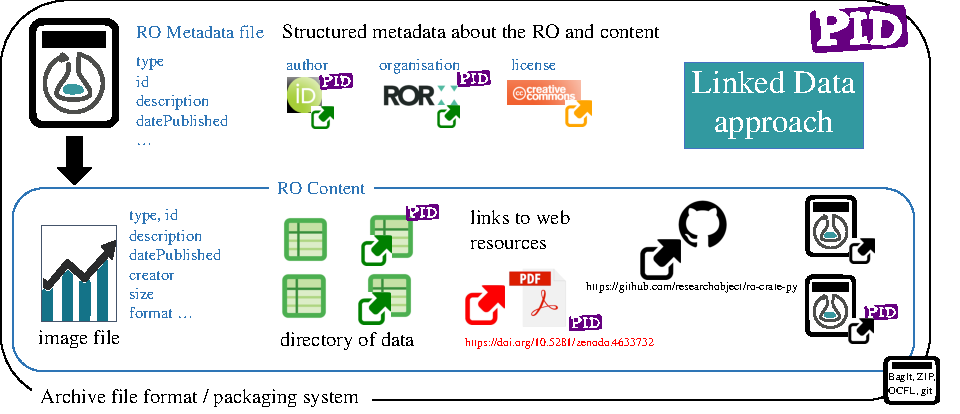
\includegraphics[width=\textwidth]{figures/ch05/ro-crate-overview.pdf}
	\caption[Conceptual overview of RO-Crate]{\textbf{Conceptual overview of RO-Crate}. A \emph{Persistent
  Identifier} (PID) \cite{McMurry 2017} points to a
  \emph{Research Object} (RO), which may be archived using different
  packaging approaches like BagIt \cite{Kunze 2018}, OCFL \cite
  {OCFL 2020}, git or ZIP. The RO is described within a \emph{RO-Crate
  Metadata File}, providing identifiers for \emph{authors} using ORCID,
  \emph{organisations} using Research Organization Registry (ROR) 
  \cite{Lammey 2020} and licences such as Creative Commons using SPDX
  identifiers. The \emph{RO-Crate content} is further described with
  additional metadata following a Linked Data approach. Data can be
  embedded files and directories, as well as links to external Web
  resources, PIDs and nested RO-Crates.}
  \label{ch5:fig:conceptual}
\end{figure}

\paragraph{Linked Data as a foundation}\label{ch5:linkeddata}

The \textbf{Linked Data} principles \cite{Bizer 2011}
(use of IRIs\footnote{\textbf{IRI}s \cite{Dürst 2005} are a generalisation
 of \textit{URI}s
(which include well-known http/https URLs), permitting international
Unicode characters without percent encoding, commonly used on the
browser address bar and in HTML5.} to identify resources (i.e. artefacts), resolvable via
HTTP, enriched with metadata and linked to each other) are core to
RO-Crate; therefore IRIs are used to identify an RO-Crate, its
constituent parts and metadata descriptions, and the properties and
classes used in the metadata.

RO-Crates are \emph{self-described} and follow the Linked Data
principles to describe all of their resources in both human and machine
readable manner. Hence, resources are identified using global
identifiers (absolute IRIs) where possible; and relationships between
two resources are defined with links.

The foundation of Linked Data and shared vocabularies also means that
multiple RO-Crates and other Linked Data resources can be indexed,
combined, queried, validated or transformed using existing Semantic Web
technologies such as SPARQL,\footnote{\url{https://www.w3.org/TR/sparql11-overview}}
SHACL\footnote{\url{https://www.w3.org/TR/shacl/}} and well established \textit{knowledge
graph} triple stores like Apache Jena\footnote{\url{https://jena.apache.org/}} and
OntoText GraphDB.\footnote{\url{https://www.ontotext.com/products/graphdb/}}

The possibilities of consuming\footnote{Some consideration is needed in processing of RO-Crates as
knowledge graphs, e.g. establishing absolute IRIs for files inside a
ZIP archive, detailed in the RO-Crate specification: \url
{https://www.researchobject.org/ro-crate/1.1/appendix/relative-uris.html}.} RO-Crate metadata with such
powerful tools gives another strong reason for using Linked Data as a
foundation. This use of mature Web\footnote{Note that an RO-Crate is not required to be published on the
Web, see Section~\vref{ch5:selfdescribed}.} technologies also means its
developers and consumers are not restricted to the Research Object
aspects that have already been specified by the RO-Crate community, but
can extend and integrate RO-Crate in multiple standardised ways.


\paragraph{RO-Crate is a self-described container}\label{ch5:selfdescribed}

An RO-Crate is defined\footnote{\url{https://www.researchobject.org/ro-crate/1.1/structure.html\#ro-crate-metadata-file-ro-crate-metadatajson}} as a self-described \textbf{Root Data Entity} that describes
and contains \emph{data entities}, which are further described by
referencing \emph{contextual entities}. A \textbf{data entity} is either
a \emph{file} (i.e.~a byte sequence stored on disk somewhere) or a
\emph{directory} (i.e.~set of named files and other directories). A file
does not need to be stored inside the RO-Crate root, it can be
referenced via a PID/IRI. A \textbf{contextual entity} exists outside
the information system (e.g.~a Person, a workflow language) and is
stored solely by its metadata. The representation of a \emph{data
entity} as a byte sequence makes it possible to store a variety of
research artefacts including not only data but also, for instance,
software and text.


The Root Data Entity is a directory, the \emph{RO-Crate Root},
identified by the presence of the \textbf{RO-Crate Metadata File}
\texttt{ro-crate-metadata.json} (top of Figure \vref{ch5:fig:conceptual}). This file describes the
RO-Crate using Linked Data, its content and related metadata using
Linked Data in JSON-LD format \cite{Sporny 2014}. This
is a W3C standard RDF serialisation that has become popular; it is easy
to read by humans while also offering some advantages for data exchange
on the Internet. JSON-LD, a subset of the widely supported and
well-known JSON format, has tooling available for many programming languages.\footnote{\url{https://json-ld.org/\#developers}}

The minimal requirements for the root data entity
metadata\footnote{\url{https://www.researchobject.org/ro-crate/1.1/root-data-entity.html\#direct-properties-of-the-root-data-entity}}
are \texttt{name}, \texttt{description} and \texttt{datePublished}, as well as a contextual
entity identifying its \texttt{license} -- additional metadata are commonly
added to entities depending on the purpose of the particular RO-Crate.

RO-Crates can be stored, transferred or published in multiple ways,
e.g.~BagIt \cite{Kunze 2018}, Oxford
Common File Layout \cite{OCFL 2020} (OCFL),
downloadable ZIP archives in Zenodo or through dedicated online
repositories, as well as published directly on the Web, e.g.~using
GitHub Pages.\footnote{\url{https://pages.github.com/}} Combined with Linked Data identifiers, this caters for a diverse set of storage and access
requirements across different scientific domains, from metagenomics
workflows producing hundreds of gigabytes of genome data to cultural
heritage records with access restrictions for personally identifiable
data. Specific \emph{RO-Crate profiles} (Section~\vref{ch5:profiles}) may constrain serialization
and publication expectations, and require additional contextual types
and properties.

\paragraph{Data Entities are described using Contextual
Entities}\label{ch5:contextualentities}

RO-Crate distinguishes between data and contextual
entities\footnote{\url{https://www.researchobject.org/ro-crate/1.1/contextual-entities.html\#contextual-vs-data-entities}} in a similar way to HTTP terminology's early
attempt to separate \emph{information} (data) and \emph{non-information}
(contextual) resources \cite{W3C 2007}. Data entities are usually files and directories located by relative IRI
references within the RO-Crate Root, but they can also be Web resources
or restricted data identified with absolute IRIs, including
\emph{Persistent Identifiers} (PIDs)
\cite{McMurry 2017}.

As both types of entities are identified by IRIs, their distinction is
allowed to be blurry; data entities can be located anywhere and be
complex, while contextual entities can have a Web presence beyond their
description inside the RO-Crate. For instance
\texttt{https://orcid.org/0000-0002-1825-0097} is primarily an
identifier for a person, but secondarily it is also a Web page and a way
to refer to their academic work.

A particular IRI may appear as a contextual entity in one RO-Crate and
as a data entity in another; the distinction lies in the fact that data
entities can be considered to be \emph{contained} or captured by that
RO-Crate (\textit{RO Content} in Figure \vref{ch5:fig:conceptual}), 
while contextual entities mainly \emph{explain} an RO-Crate or its
content (although this distinction is not a formal requirement).

In RO-Crate, a referenced contextual entity (e.g.~a person identified by
ORCID) should always be described within the RO-Crate Metadata File with
at least a \emph{type} and \emph{name}, even where their PID might
resolve to further Linked Data. This is so that clients are not required
to follow every link for presentation purposes, for instance HTML
rendering. Similarly any imported extension
terms\footnote{\url{https://www.researchobject.org/ro-crate/1.1/appendix/jsonld.html\#extending-ro-crate}} would themselves also have a human-readable description in the
case where their PID does not directly resolve to human-readable
documentation.

Figure \vref{ch5:fig:uml} shows a simplified class
diagram of RO-Crate, highlighting the different types of data entities
and contextual entities that can be aggregated and related. While an
RO-Crate would usually contain one or more data entities
(\texttt{hasPart}), it may also be a pure aggregation of contextual
entities (\texttt{mentions}).

\begin{figure}
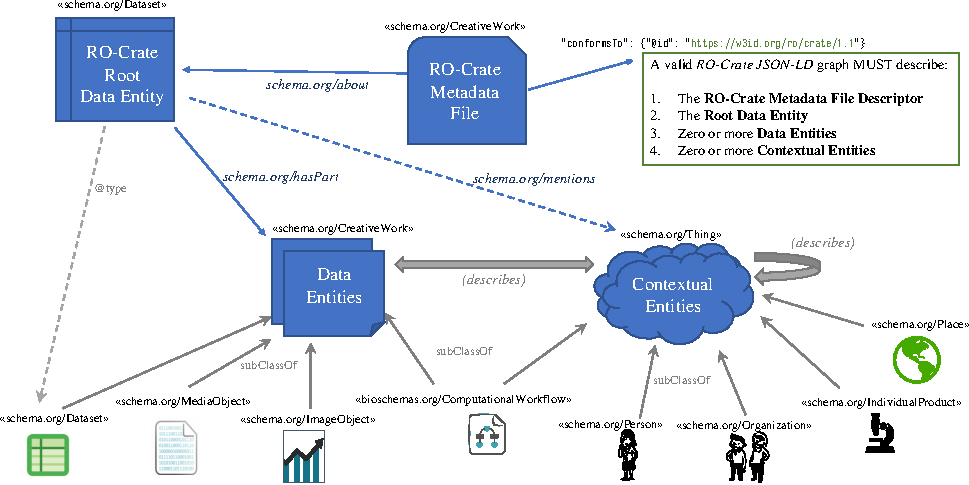
\includegraphics[width=\textwidth]{figures/ch05/ro-crate-uml.pdf}
	\caption[Simplified class diagram of RO-Crate]{\textbf{Simplified class diagram of RO-Crate}. The 
\emph{RO-Crate Metadata File} conforms to a version of the specification;
and contains a JSON-LD graph \cite{Sporny 2014} that describes the
entities that make up the RO-Crate. The \emph{RO-Crate Root Data
Entity} represent the Research Object as a dataset. The RO-Crate
aggregates \emph{data entities} (\texttt{hasPart}) which are further
described using \emph{contextual entities} (which may include
aggregated and non-aggregated data entities). Multiple types and
relations from schema.org allow annotations to be more specific,
including figures, nested datasets, computational workflows, people,
organisations, instruments and places. Contextual entities not
otherwise cross-referenced from other entities' properties 
(\emph{describes}) can be grouped under the root entity (\texttt{mentions}).}
\label{ch5:fig:uml}
\end{figure}

\paragraph{Guide through Recommended
Practices}\label{ch5:recommendedpractices}

RO-Crate as a specification aims to build a set of recommended practices
on how to practically apply existing standards in a common way to
describe research outputs and their provenance, without having to learn
each of the underlying technologies in detail.

As such, the RO-Crate 1.1
specification\footnote{\url{https://w3id.org/ro/crate/1.1}} \cite{RO-Crate 1.1.3}
can be seen as an opinionated and example-driven guide to writing
\footurl{https://schema.org/}{schema.org}
\cite{Guha 2015} metadata as
JSON-LD \cite{Sporny 2014} (see
section \vref{ch5:implementation}), which
leaves it open for implementers to include additional metadata using
other schema.org types and properties, or even additional Linked Data
vocabularies/ontologies or their own ad-hoc terms.

However the primary purpose of the RO-Crate specification is to assist
developers in leveraging Linked Data principles for the focused purpose
of describing Research Objects in a structured language, while reducing
the steep learning curve otherwise associated with Semantic Web
adaptation, like development of ontologies, identifiers, namespaces, and
RDF serialization choices.

\subsubsection{Ensuring Simplicity}\label{ch5:simplicity}

One aim of RO-Crate is to be conceptually simple. This simplicity has
been repeatedly checked and confirmed through an informal community
review process. For instance, in the discussion on supporting ad-hoc
vocabularies\footnote{\url{https://github.com/ResearchObject/ro-crate/issues/71}} in
RO-Crate, the community explored potential Linked Data solutions. The
conventional wisdom in RDF best
practices\footnote{\url{https://www.w3.org/TR/swbp-vocab-pub/}} is to establish a
vocabulary with a new IRI namespace, formalised using RDF
Schema\footnote{\url{http://www.w3.org/TR/2014/REC-rdf-schema-20140225/}} or
OWL\footnote{\url{http://www.w3.org/TR/2012/REC-owl2-overview-20121211/}}
ontologies. However, this may seem an excessive learning curve for
non-experts in semantic knowledge representation, and the RO-Crate
community instead agreed on a dual lightweight approach: (i)
Document\footnote{\url{https://www.researchobject.org/ro-crate/1.1/appendix/jsonld.html\#adding-new-or-ad-hoc-vocabulary-terms}}
how projects with their own Web-presence can make a pure HTML-based
vocabulary, and (ii) provide a community-wide PID namespace under
\texttt{https://w3id.org/ro/terms} that redirect to simple CSV files
maintained in GitHub.\footnote{\url{https://github.com/ResearchObject/ro-terms}}

To further verify this idea of simplicity, we have formalised the
RO-Crate definition (see \textit{section ~\vref{ch5:formaldefinition}}). An
important result of this exercise is that the underlying data structure
of RO-Crate, although conceptually a graph, is represented as a
depth-limited tree. This formalisation also emphasises the
\textit{boundedness} of the structure; namely, the fact that elements are
specifically identified as being either semantically \textit{contained} by the
RO-Crate as \textit{Data Entities} (\texttt{hasPart}) or mainly referenced
(\texttt{mentions}) and typed as \textit{external} to the Research Object as
\textit{Contextual Entities}. It is worth pointing out that this semantic
containment can extend beyond the physical containment of files
residing within the RO-Crate Root directory on a given storage system,
as the RO-Crate data entities may include any data resource globally
identifiable using IRIs.

\subsubsection{Extensibility and RO-Crate profiles}\label{ch5:profiles}

The RO-Crate specification provides a core set of conventions to
describe research outputs using types and properties applicable across
scientific domains. However we have found that domain-specific use of
RO-Crate will, implicitly or explicitly, form a specialised
\textbf{profile} of RO-Crate; i.e., \emph{a set of conventions, types
and properties that are minimally required and one can expect to be
present in that subset of RO-Crates}. For instance, RO-Crates used for
exchange of workflows will have to contain a data entity of type
\texttt{ComputationalWorkflow}, or cultural heritage records should have
a \texttt{contentLocation}.

Making such profiles explicit allow further reliable programmatic
consumption and generation of RO-Crates beyond the core types defined in
the RO-Crate specification. Following the RO-Crate mantra of
\emph{guidance over strictness}, profiles are mainly \emph{duck-typing}
rather than strict syntactic or semantic types, but may also have
corresponding machine-readable schemas at multiple levels (file formats,
JSON, RDF shapes, RDFS/OWL semantics).

The next version of the RO-Crate specification 1.2 will define a
formalization\footnote{\url{https://www.researchobject.org/ro-crate/1.2-DRAFT/profiles}}
for publishing and declaring conformance to RO-Crate profiles. Such a
profile is primarily a human-readable document of before-mentioned
expectations and conventions, but may also define a machine-readable
profile as a \textbf{Profile Crate}: Another RO-Crate that describe the
profile and in addition can list schemas for validation, compatible
software, applicable repositories, serialization/packaging formats,
extension vocabularies, custom JSON-LD contexts and examples (see for
example the Workflow RO-Crate
profile\footnote{\url{https://w3id.org/workflowhub/workflow-ro-crate/}}).


In addition, there are sometimes existing domain-specific metadata
formats, but they are either not RDF-based (and thus time-consuming to
construct terms for in JSON-LD) or are at a different granularity level
that might become overwhelming if represented directly in the RO-Crate
Metadata file (e.g.~W3C PROV bundle detailing every step execution of a
workflow run
\cite{Khan 2019}). RO-Crate
allows such \emph{alternative metadata files} to co-exist, and be
described as data entities with references to the standards and
vocabularies they conform to. This simplifies further programmatic
consumption even where no filename or file extension conventions have
emerged for those metadata formats.

Section \vref{ch5:inuse} examines the observed
specializations of RO-Crate use in several domains and their emerging
profiles.

\subsubsection{Technical implementation of the RO-Crate
model}\label{ch5:implementation}

The RO-Crate conceptual model has been realised using JSON-LD and
schema.org in a prescriptive form as discussed in Section~\vref{ch5:conceptual}. These technical
choices were made to cater for simplicity from a developer perspective
(as introduced in Section~\vref{ch5:methodology}).

JSON-LD\footnote{\url{https://json-ld.org/}} \cite{Sporny 2014}
provides a way to express Linked Data as a JSON structure, where a
\emph{context} provides mapping to RDF properties and classes. While
JSON-LD cannot map arbitrary JSON structures to RDF, we found that it
does lower the barrier compared to other RDF syntaxes, as the JSON
syntax nowadays is a common and popular format for data exchange on the
Web.

However, JSON-LD alone has too many degrees of freedom and hidden
complexities for software developers to reliably produce and consume
without specialised expertise or large RDF software frameworks. A large
part of the RO-Crate specification is therefore dedicated to describing
the acceptable subset of JSON structures.

\paragraph{RO-Crate JSON-LD}\label{ch5:jsonld}

RO-Crate
mandates\footnote{\url{https://www.researchobject.org/ro-crate/1.1/appendix/jsonld.html}}
the use of flattened, compacted JSON-LD in the RO-Crate Metadata file
\texttt{ro-crate-metadata.json}\footnote{The avid reader may spot that the RO-Crate Metadata file use the
extension \texttt{.json} instead of \texttt{.jsonld}, this is to emphasise the
developer expectations as a JSON format, while the file's JSON-LD
nature is secondary. See \url
{https://github.com/ResearchObject/ro-crate/issues/82}.}
where a single \texttt{@graph} array contains all
the data and contextual entities in a flat list. An example can be seen
in the JSON-LD snippet in Listing \vref{ch5:lis1}, describing a simple RO-Crate
containing data entities described using contextual entities.

\begin{listing}
  \footnotesize
  \begin{verbatim}
  { "@context": "https://w3id.org/ro/crate/1.1/context",
    "@graph": [
      { "@id": "ro-crate-metadata.json",      
        "@type": "CreativeWork",
        "conformsTo": {"@id": "https://w3id.org/ro/crate/1.1"},
        "about": {"@id": "./"}
      },
      { "@id": "./",
        "@type": "Dataset",
        "name": "A simplified RO-Crate",
        "author": {"@id": "#alice"},
        "license": {"@id": "https://spdx.org/licenses/CC-BY-4.0"},
        "datePublished": "2021-11-02T16:04:43Z",
        "hasPart": [
          {"@id": "survey-responses-2019.csv"},
          {"@id": "https://example.com/pics/5707039334816454031_o.jpg"}
        ]
      },
      { "@id": "survey-responses-2019.csv",
        "@type": "File",
        "about": {"@id": "https://example.com/pics/5707039334816454031_o.jpg"},
        "author": {"@id": "#alice"}
      },
      { "@id": "https://example.com/pics/5707039334816454031_o.jpg",
        "@type": ["File", "ImageObject"],
        "contentLocation": {"@id": "http://sws.geonames.org/8152662/"},
        "author": {"@id": "https://orcid.org/0000-0002-1825-0097"}
      },
      { "@id": "#alice",
        "@type": "Person",
        "name": "Alice"
      },
      { "@id": "https://orcid.org/0000-0002-1825-0097",
        "@type": "Person",
        "name": "Josiah Carberry"
      },
      { "@id": "http://sws.geonames.org/8152662/",
        "@type": "Place",
        "name": "Catalina Park"
      },
      { "@id": "https://spdx.org/licenses/CC-BY-4.0",
        "@type": "CreativeWork",
        "name": "Creative Commons Attribution 4.0"
      }
    ]
  }    
  \end{verbatim}    
	\caption[Simplified RO-Crate metadata file]{%\qq{}\protect\footnotemark[31]
  Simplified\footnotemark RO-Crate metadata file showing the
  flattened compacted JSON-LD \texttt{@graph} array containing the data entities
  and contextual entities, cross-referenced using \texttt{@id}. The
  \texttt{ro-crate-metadata.json} entity self-declares conformance with the
  RO-Crate specification using a versioned persistent identifier, further
  RO-Crate descriptions are on the root data entity \texttt{./} or any of the
  referenced data or contextual entities. This is exemplified by the data
  entity \texttt{ImageObject} referencing contextual entities for
  \texttt{contentLocation} and \texttt{author} that differs from that of the overall
  RO-Crate. In this crate, \texttt{about} of the CSV data entity reference the
  \texttt{ImageObject}, which then take the roles of both a data entity and
  contextual entity. While \texttt{Person} entities ideally are identified with
  ORCID PIDs as for Josiah, \texttt{\#alice} is here in contrast an RO-Crate
  local identifier, highlighting the pragmatic ``just enough'' Linked
  Data approach.}
  \label{ch5:lis1}
\end{listing}
  
\footnotetext{
    Recommended properties for types shown in
    listing also include
    \texttt{affiliation}, \texttt{citation}, \texttt{contactPoint},
    \texttt{description},
    \texttt{encodingFormat}, \texttt{funder}, \texttt{geo}, \texttt{identifier},
    \texttt{keywords},
    \texttt{publisher}; these properties and corresponding contextual
    entities are
    excluded here for brevity. See complete example
    \url
    {https://www.researchobject.org/2021-packaging-research-artefacts-with-ro-crate/listing1/}.
}
 

In this flattened profile of JSON-LD, each \texttt{\{entity\}} are
directly under \texttt{@graph} and represents the RDF triples with a
common \emph{subject} (\texttt{@id}), mapped \emph{properties} like
\texttt{hasPart}, and \emph{objects} --- as either literal
\texttt{"string"} values, referenced \texttt{\{objects\}} (which
properties are listed in its own entity), or a JSON \texttt{{[}list{]}}
of these. If processed as JSON-LD, this forms an RDF graph by matching
the \texttt{@id} IRIs and applying the \texttt{@context} mapping to
schema.org terms. \normalsize

\paragraph{Flattened JSON-LD}\label{ch5:flattened-json-ld}

When JSON-LD 1.0 \cite{Sporny 2014}
was
proposed, one of the motivations was to seamlessly apply an RDF nature
on top of regular JSON as frequently used by Web APIs. JSON objects in
APIs are frequently nested with objects at multiple levels, and the
perhaps most common form of JSON-LD is the compacted
form\footnote{\url{https://json-ld.org/spec/REC/json-ld/20140116/\#compacted-document-form}}
which follows this expectation (JSON-LD
1.1\footnote{\url{https://www.w3.org/TR/2020/REC-json-ld11-20200716/}} further
expands these capabilities, e.g. allowing nested \texttt{@context} definitions).


While this feature of JSON-LD can be seen as a way to ``hide'' its RDF
nature, we found that the use of nested trees (e.g.~a \texttt{Person}
entity appearing as \texttt{author} of a \texttt{File} which nests under
a \texttt{Dataset} with \texttt{hasPart}) counter-intuitively forces
consumers to consider the JSON-LD as an RDF Graph, since an identified
\texttt{Person} entity can appear at multiple and repeated points of the
tree (e.g.~author of multiple files), necessitating node merging or
duplication, which can become complicated as this approach also invites
the use of \emph{blank nodes} (entities missing \texttt{@id}).

By comparison, a single flat \texttt{@graph} array approach, as required
by RO-Crate, means that applications can choose to process and edit each
entity as pure JSON by a simple lookup based on \texttt{@id}. At the
same time, lifting all entities to the same level reflects the Research
Object principles
\cite{Bechhofer 2013}
in that describing the context and provenance is just as important as
describing the data, and the requirement of \texttt{@id} of every entity
forces RO-Crate generators to consciously
consider
existing IRIs and identifiers.\footnote{\url{https://www.researchobject.org/ro-crate/1.1/appendix/jsonld.html\#describing-entities-in-json-ld}}

\paragraph{JSON-LD context}\label{ch5:json-ld-context}

In JSON-LD, the \texttt{@context} is a reference to another JSON-LD
document that provides mapping from JSON keys to Linked Data term IRIs,
and can enable various JSON-LD directives to cater for customised JSON
structures for translating to RDF.

RO-Crate reuses vocabulary terms and IRIs from schema.org, but provides
its own versioned JSON-LD
context,\footnote{\url{https://w3id.org/ro/crate/1.1/context}} which has a flat list
with the mapping from JSON-LD keys to their IRI equivalents (e.g. key
\texttt{"author"} maps to the \url{http://schema.org/author} property).

The rationale behind this decision is to support JSON-based RO-Crate
applications that are largely unaware of JSON-LD, that still may want to
process the \texttt{@context} to find or add Linked Data definitions of
otherwise unknown properties and types. Not reusing the official
schema.org context means RO-Crate is also able to map in additional
vocabularies where needed, namely the \emph{Portland Common Data Model}
(PCDM) \cite{Cossu 2018}
for
repositories and Bioschemas \cite{Gray 2017}
for
describing computational workflows. RO-Crate profiles may
extend\footnote{\url{https://www.researchobject.org/ro-crate/1.1/appendix/jsonld.html\#extending-ro-crate}}
the \texttt{@context} to re-use additional domain-specific ontologies.


Similarly, while the schema.org context
currently\footnote{\url{https://schema.org/version/13.0/schemaorg-current-http.jsonld}}
have \texttt{"@type": "@id"} annotations for implicit object properties, RO-Crate
JSON-LD distinguishes explicitly between references to other entities
\texttt{\{"@id": "\#alice"}\}
and string values \texttt{"Alice"} -- meaning
RO-Crate applications can find references for corresponding entities
and IRIs without parsing the \texttt{@context} to understand a particular
property. Notably this is exploited by the \textit{ro-crate-html-js}
\cite{ro-crate-html-js} tool to provide reliable HTML rendering for
otherwise unknown properties and types.

\subsubsection{RO-Crate Community}\label{ch5:community}

The RO-Crate conceptual model, implementation and best practices are
developed by a growing community of researchers, developers and
publishers. RO-Crate's community is a key aspect of its effectiveness in
making research artefacts FAIR. Fundamentally, the community provides
the overall context of the implementation and model and ensures its
interoperability.

The RO-Crate community consists of:

\begin{enumerate}
\item
  A diverse set of people representing a variety of stakeholders.
\item
  A set of collective norms.
\item
  An open platform that facilitates communication (GitHub, Google Docs,
  monthly teleconferences).
\end{enumerate}

\hypertarget{people}{%
\paragraph{People}\label{ch5:people}}

The initial concept of RO-Crate was formed at the first Workshop on
Research Objects\footnote{\url{https://www.researchobject.org/ro2018/}} (RO2018),
held as part of the IEEE conference on eScience. This workshop followed
up on considerations made at a Research Data Alliance (RDA) meeting on
Research Data
Packaging\footnote{\url{https://rd-alliance.org/approaches-research-data-packaging-rda-11th-plenary-bof-meeting}}
that found similar goals across multiple data packaging efforts
\cite{Ó Carragáin 2019a}: simplicity, structured metadata and the
use of JSON-LD.

An important outcome of discussions that took place at RO2018 was the
conclusion that the original Wf4Ever Research Object ontologies
\cite{Belhajjame 2015}, in
principle sufficient for packaging research artefacts with rich
descriptions, were, in practice, considered inaccessible for regular
programmers (e.g., Web developers) and in danger of being
incomprehensible for domain scientists due to their reliance on Semantic
Web technologies and other ontologies.

DataCrate \cite{Sefton 2018} was
presented at RO2018 as a promising lightweight alternative approach, and
an agreement was made by a group of volunteers to attempt building what
was initially called \emph{``RO Lite''} as a combination of DataCrate's
implementation and Research Object's principles.

This group, originally made up of library and Semantic Web experts, has
subsequently grown to include domain scientists, developers, publishers
and more. This perspective of multiple views led to the specification
being used in a variety of domains, from bioinformatics and regulatory
submissions to humanities and cultural heritage preservation.

The RO-Crate community is strongly engaged with the European-wide
biology/bioinformatics collaborative e-Infrastructure ELIXIR
\cite{Crosswell 2012}, along with European Open Science
Cloud\footnote{\url{https://eosc.eu/}} (EOSC) projects including
EOSC-Life,\footnote{\url{https://www.eosc-life.eu/}}
FAIRplus,\footnote{\url{https://fairplus-project.eu/}}
CS3MESH4EOSC\footnote{\url{https://cs3mesh4eosc.eu/}} and
BY-COVID.\footnote{\url{https://by-covid.eu/}} RO-Crate has also established
collaborations with Bioschemas \cite{Gray 2017}, GA4GH
\cite{Rehm 2021}, OpenAIRE \cite{Rettberg 2015}
and multiple H2020 projects.

A key set of stakeholders are developers: the RO-Crate community has
made a point of attracting developers who can implement the
specifications but, importantly, keeps ``developer user experience'' in
mind. This means that the specifications are straightforward to
implement and thus do not require expertise in technologies that are not
widely deployed.

This notion of catering to ``developer user experience'' is an example
of the set of norms that have developed and now define the community.

\paragraph{Norms}\label{ch5:norms}

The RO-Crate community is driven by informal conventions and notions
that are prevalent but not neccessarily written down. Here, we distil
what we as authors believe are the critical set of norms that have
facilitated the development of RO-Crate and contributed to the ability
for RO-Crate research packages to be FAIR. This is not to say that there
are no other norms within the community nor that everyone in the
community holds these uniformly. Instead, what we emphasise is that
these norms are helpful and also shaped by community practices:

\begin{enumerate}
\item
  Simplicity.
\item
  Developer friendliness.
\item
  Focus on examples and best practices rather than rigorous
  specification.
\item
  Reuse ``just enough'' Web standards.
\end{enumerate}

A core norm of RO-Crate is that of \textbf{simplicity}, which sets the
scene for how we guide developers to structure metadata with RO-Crate.
We focus mainly on documenting simple approaches to the most common use
cases, such as authors having an affiliation. This norm also influences
our take on \textbf{developer friendliness}; for instance, we are using
the Web-native JSON format, allowing only a few of JSON-LD's flexible
Linked Data features. Moreover, the RO-Crate documentation is largely
built up by \textbf{examples} showcasing \textbf{best practices}, rather
than rigorous specifications. We build on existing \textbf{Web
standards} that themselves are defined rigorously, which we utilise
\emph{``\textbf{just enough}''} in order to benefit from the advantages
of Linked Data (e.g., extensions by namespaced vocabularies), without
imposing too many developer choices or uncertainties (e.g., having to
choose between the many RDF syntaxes).

While the above norms alone could easily lead to the creation of ``yet
another'' JSON format, we keep the goal of \textbf{FAIR
interoperability} of the captured metadata, and therefore follow closely
FAIR best practices and current developments such as data citations,
PIDs, open repositories and recommendations for sharing research outputs
and software.

\paragraph{Open Platforms}\label{ch5:open-platforms}

The critical infrastructure that enables the community around RO-Crate
is the use of open development platforms. This underpins the importance
of open community access to supporting FAIR. Specifically, it is
difficult to build and consume FAIR research artefacts without being
able to access the specifications, understand how they are developed,
know about any potential implementation issues, and discuss usage to
evolve best practices.

The development of RO-Crate was driven by capturing documentation of
real-life examples and best practices rather than creating a rigorous
specification. At the same time, we agreed to be opinionated on the
syntactic form to reduce the jungle of implementation choices; we wanted
to keep the important aspects of Linked Data to adhere to the FAIR
principles while retaining the option of combining and extending the
structured metadata using the existing Semantic Web stack, not just
build a standalone JSON format.

Further work during 2019 started adapting the DataCrate documentation
through a more collaborative and exploratory \emph{RO Lite} phase,
initially using Google Docs for review and discussion, then moving to
GitHub as a collaboration space for developing what is now the RO-Crate
specification, maintained\footnote{\url{https://github.com/researchobject/ro-crate/}} as
Markdown in GitHub Pages
and published through Zenodo.

In addition to the typical Open Source-style development with GitHub
issues and pull requests, the RO-Crate Community have, at time of
writing, two regular monthly calls, a Slack channel and a mailing list
for coordinating the project; also many of its participants collaborate
on RO-Crate at multiple conferences and coding events such as the
ELIXIR BioHackathon.\footnote{\url{https://biohackathon-europe.org/}} The community
is jointly developing the RO-Crate specification and Open Source tools,
as well as providing support and considering new use cases. The
RO-Crate Community\footnote{\url{https://www.researchobject.org/ro-crate/community}}
is open for anyone to join, to equally participate under a code of
conduct, and as of October 2021 has more than 50 members (see \vref{ro-crate-community}).

\subsection{RO-Crate Tooling}\label{ch5:tooling}

The work of the community has led to the development of a number of
tools for creating and using RO-Crates. Table \vref{ch5:tab1} shows the current set
of implementations\footnote{
  Several new implementations have appeared since the publication of this article, see section \vref{ch61:rocratefuture}.
}. Reviewing this list, one can see support for
commonly used programming languages, including Python, JavaScript, and
Ruby. Additionally, the tools can be integrated into commonly used
research environments, in particular, the command line tool
\textit{ro-crate-html-js} \cite{ro-crate-html-js} for creating a human-readable
preview of an RO-Crate as a sidecar HTML file. Furthermore, there are
tools that cater to end-users (\textit{Describo} \cite{La Rosa 2021d}, \textit{WorkflowHub}
\cite{WorkflowHub 2023}), in order to simplify creating and managing
RO-Crate. For example, Describo was developed to help researchers of
the Australian Criminal Characters
project\footnote{\url{https://criminalcharacters.com/}} to annotate historical prisoner
records for greater insight into the history of Australia
\cite{Piper 2020}.

While the development of these tools is promising, our analysis of their
maturity status shows that the majority of them are in the Beta stage.
This is partly due to the fact that the RO-Crate specification itself
only recently reached 1.0 status, in November 2019
\cite{RO-Crate 1.0}. Now that there
is a fixed point of reference: With version 1.1 (October 2020)
\cite{RO-Crate 1.1} RO-Crate has
stabilised based on feedback from application development, and now we
are seeing a further increase in the maturity of these tools, along with
the creation of new ones.

Given the stage of the specification, these tools have been primarily
targeting developers, essentially providing them with the core libraries
for working with RO-Crate. Another target has been that of research data
managers who need to manage and curate large amounts of data.

\small
\begin{longtable}[]{@{}
>{\raggedright\arraybackslash}p{(\columnwidth - 8\tabcolsep) * \real{0.21}}
>{\raggedright\arraybackslash}p{(\columnwidth - 8\tabcolsep) * \real{0.11}}
>{\raggedright\arraybackslash}p{(\columnwidth - 8\tabcolsep) * \real{0.19}}
>{\raggedright\arraybackslash}p{(\columnwidth - 8\tabcolsep) * \real{0.09}}
>{\raggedright\arraybackslash}p{(\columnwidth - 8\tabcolsep) * \real{0.40}}@{}}
\caption[Applications and libraries implementing RO-Crate]{{\bf Applications and libraries implementing RO-Crate}, targeting
  different types of users across multiple programming languages. Status
  is indicative as assessed by this work (Alpha \textless{} Beta
  \textless{} Release Candidate (RC) \textless{} Release).
}
\label{ch5:tab1}\tabularnewline
\toprule
Tool Name & Targets & Language /Platform & Status & Brief Description \\
\midrule
\endhead
Describo \cite{La Rosa 2021d} &
Research Data Managers & NodeJS (Desktop) & RC & Interactive desktop
application to create, update and export RO-Crates for different
profiles \\
Describo Online
\cite{La Rosa 2021c} &
Platform developers & NodeJS (Web) & Alpha & Web-based application to
create RO-Crates using cloud storage \\
ro-crate-excel
\cite{Lynch 2022} & Data
managers & JavaScript & Beta & Command-line tool to create/edit
RO-Crates with spreadsheets \\
ro-crate-html-js
\cite{ro-crate-html-js} &
Developers & JavaScript & Beta & HTML rendering of RO-Crate \\
ro-crate-js
\cite{Sefton 2021b} & Research
Data Managers & JavaScript & Alpha & Library for creating/manipulating
crates; basic validation code \\
ro-crate-ruby
\cite{Bacall 2022b} &
Developers & Ruby & Beta & Ruby library for reading/writing RO-Crate,
with workflow support \\
ro-crate-py \cite{De Geest 2023a}) &
Developers & Python & Alpha & Object-oriented Python library for
reading/writing RO-Crate and use by Jupyter Notebook \\
WorkflowHub \cite{WorkflowHub 2023} & Workflow
users & Ruby & Beta & Workflow repository; imports and exports Workflow
RO-Crate \\
Life Monitor \cite{CRS4 2022} & Workflow
developers & Python & Alpha & Workflow testing and monitoring service;
Workflow Testing profile of RO-Crate \\
SCHeMa \cite{Vergoulis 2022} & Workflow
users & PHP & Alpha & Workflow execution using RO-Crate as exchange
mechanism
\cite{Vergoulis 2021} \\
galaxy2cwl \cite{Eguinoa 2020}
& Workflow developers & Python & Alpha & Wraps Galaxy workflow as
Workflow RO-Crate \\
Modern PARADISEC \cite{La Rosa 2021a} &
Repository managers & Platform & Beta & Cultural Heritage portal based
on OCFL and RO-Crate \\
ONI express
\cite{Arkisto 2022} &
Repository managers & Platform & Beta & Platform for publishing data and
documents stored in an OCFL repository via a Web interface \\
ocfl-tools \cite{La Rosa 2021b} &
Developers & JavaScript (CLI) & Beta & Tools for managing RO-Crates in
an OCFL repository \\
RO Composer
\cite{Bacall 2019} &
Repository developers & Java & Alpha & REST API for gradually building
ROs for given profile. \\
RDA maDMP Mapper \cite{Arfaoui 2020}
& Data Management Plan users & Python & Beta & Mapping between
machine-actionable data management plans (maDMP) and RO-Crate
\cite{Miksa 2020} \\
Ro-Crate\_2\_ma-DMP
\cite{Brenner 2020} & Data
Management Plan users & Python & Beta & Convert between
machine-actionable data management plans (maDMP) and RO-Crate \\
CheckMyCrate
\cite{Belchev 2021} &
Developers & Python (CLI) & Alpha & Validation according to Workflow
RO-Crate profile \\
RO-Crates-and-Excel
\cite{Zoubek 2021} & Data Managers
& Java (CLI) & Alpha & Describe column/data details of spreadsheets as
RO-Crate using DataCube vocabulary \\
\bottomrule

\end{longtable}

\normalsize


\subsection{Profiles of RO-Crate in use}\label{ch5:inuse}

RO-Crate fundamentally forms part of an infrastructure to help build
FAIR research artefacts. In other words, the key question is whether
RO-Crate can be used to share and (re)use research artefacts. Here we
look at three research domains where RO-Crate is being applied:
Bioinformatics, Regulatory Science and Cultural Heritage. In addition,
we note how RO-Crate may have an important role as part of
machine-actionable data management plans and institutional repositories.

From these varied uses of RO-Crate we observe natural differences in
their detail level and the type of entities described by the RO-Crate.
For instance, on submission of an RO-Crate to a workflow repository, it
is reasonable to expect the RO-Crate to contain at least one workflow,
ideally with a declared licence and workflow language. Specific
additional recommendations such as on identifiers is also needed to meet
the emerging requirements of FAIR Digital
Objects.\footnote{\url{https://fairdo.org/}} Work has now
begun\footnote{\url{https://github.com/ResearchObject/ro-crate/issues/153} was implemented after publication of this article -- see section \vref{ch61:profiles}.} to
formalise these different \textit{profiles} of RO-Crates, which may impose
additional constraints based on the needs of a specific domain or use case.


\subsubsection{Bioinformatics workflows}\label{ch5:workflows}

WorkflowHub.eu\footnote{\url{https://workflowhub.eu/}} is a European cross-domain
registry of computational workflows, supported by European Open Science
Cloud projects, e.g. EOSC-Life,\footnote{\url{https://www.eosc-life.eu/}} and
research infrastructures including the pan-European bioinformatics
network ELIXIR\footnote{\url{https://elixir-europe.org/}}
\cite{Crosswell 2012}. As part
of promoting workflows as reusable tools, WorkflowHub includes
documentation and high-level rendering of the workflow structure
independent of its native workflow definition format. The rationale is
that a domain scientist can browse all relevant workflows for their
domain, before narrowing down their workflow engine requirements. As
such, the WorkflowHub is intended largely as a registry of workflows
already deposited in repositories specific to particular workflow
languages and domains, such as UseGalaxy.eu
\cite{Baker 2020} and
Nextflow nf-core
\cite{Ewels 2020}.

We here describe three different RO-Crate profiles developed for use
with WorkflowHub.

\paragraph{Profile for describing workflows}
\label{ch5:profile-for-describing-workflows}

Being cross-domain, WorkflowHub has to cater for many different workflow
systems. Many of these, for instance Nextflow
\cite{Di Tommaso 2017} and Snakemake
\cite{Köster 2012}, by
virtue of their script-like nature, reference multiple neighbouring
files typically maintained in a GitHub repository. This calls for a data
exchange method that allows keeping related files together. WorkflowHub
has tackled this problem by adopting RO-Crate as the packaging mechanism
\cite{Bietrix 2021}, typing and
annotating the constituent files of a workflow and --- crucially ---
marking up the workflow language, as many workflow engines use common
file extensions like \texttt{*.xml} and \texttt{*.json}. Workflows are
further described with authors, license, diagram previews and a listing
of their inputs and outputs. RO-Crates can thus be used for
interoperable deposition of workflows to WorkflowHub, but are also used
as an archive for downloading workflows, embedding metadata registered
with the WorkflowHub entry and translated workflow files such as
abstract Common Workflow Language (CWL)
\cite{Crusoe 2022} definitions and
diagrams \cite{Goble 2021}.

RO-Crate acts therefore as an interoperability layer between registries,
repositories and users in WorkflowHub. The iterative development between
WorkflowHub developers and the RO-Crate community heavily informed the
creation of the Bioschemas
\cite{Gray 2017} profile for Computational
Workflows \footnote{\url{https://bioschemas.org/profiles/ComputationalWorkflow/1.0-RELEASE/}}, which again informed the
RO-Crate
1.1 specification on workflows \footnote{\url{https://www.researchobject.org/ro-crate/1.1/workflows.html}} and led to the RO-Crate Python library
\cite{De Geest 2023a} and
WorkflowHub's
\textbf{Workflow
RO-Crate profile}\footnote{\url{https://w3id.org/workflowhub/workflow-ro-crate/1.0}}, which, in a similar fashion to RO-Crate itself,
recommends which workflow resources and descriptions are required. This
co-development across project boundaries exemplifies the drive for
simplicity and for establishing best practices.

\paragraph{Profile for recording workflow runs}
\label{ch5:profile-for-recording-workflow-runs}

RO-Crates in WorkflowHub have so far been focused on workflows that are
ready to be run, and development of WorkflowHub is now creating a
\textbf{Workflow Run RO-Crate profile}\footnote{Section \vref{ch54:wrroc}} for the purposes of benchmarking,
testing and executing workflows. As such, RO-Crate serves as a container
of both a \emph{workflow definition} that may be executed and of a
particular \emph{workflow execution with test results}.

This workflow run profile is a continuation of our previous work with
capturing workflow provenance in a Research Object in CWLProv
\cite{Khan 2019} and
TavernaPROV \cite{Soiland-Reyes 2016}.
In both cases, we used the PROV Ontology
\cite{Lebo 2013a},
including details of every task execution with all the intermediate
data, which required significant workflow engine integration.\footnote{CWLProv
  and TavernaProv predate RO-Crate, but use RO-Bundle
  \cite{Soiland-Reyes 2014}, a similar
  Research Object packaging method with JSON-LD metadata.}

Simplifying from the CWLProv approach, the planned Workflow Run RO-Crate
profile will use a high level schema.org
provenance\footnote{\url{https://www.researchobject.org/ro-crate/1.1/provenance.html\#software-used-to-create-files}}
for the input/output boundary of the overall workflow
execution. This \emph{Level 1 workflow provenance}
\cite{Khan 2019} can be
expressed generally across workflow languages with minimal workflow
engine changes, with the option of more detailed provenance traces as
separate PROV artefacts in the RO-Crate as data entities. In the current
development of Specimen Data
Refinery\footnote{\url{https://github.com/DiSSCo/SDR}} \cite{Walton 2020a} these
RO-Crates will document the text recognition workflow runs of digitised
biological specimens, exposed as FAIR Digital Objects
\cite{De Smedt 2020}.

WorkflowHub has recently enabled minting of Digital Object Identifiers
(DOIs), a PID commonly used for scholarly artefacts, for registered
workflows, e.g.~\texttt{10.48546/workflowhub.workflow.56.1}
\cite{Lowe 2021b},
lowering the barrier for citing workflows as computational methods along
with their FAIR metadata -- captured within an RO-Crate. While it is not
an aim for WorkflowHub to be a repository of workflow runs and their
data, RO-Crates of \emph{exemplar workflow runs} serve as useful
workflow documentation, as well as being an exchange mechanism that
preserves FAIR metadata in a diverse workflow execution environment.

\paragraph{Profile for testing workflows}\label{ch5:profile-for-testing-workflows}

The value of computational workflows, however, is potentially undermined
by the ``collapse'' over time of the software and services they depend
upon: for instance, software dependencies can change in a
non-backwards-compatible manner, or active maintenance may cease; an
external resource, such as a reference index or a database query
service, could shift to a different URL or modify its access protocol;
or the workflow itself may develop hard-to-find bugs as it is updated.
This \emph{workflow decay} can take a big toll on the workflow's
reusability and on the reproducibility of any processes it evokes
\cite{Zhao 2012}.

For this reason, WorkflowHub is complemented by a monitoring and testing
service called LifeMonitor
\cite{CRS4 2022}, also supported
by EOSC-Life. LifeMonitor's main goal is to assist in the creation,
periodic execution and monitoring of workflow tests, enabling the early
detection of software collapse in order to minimise its detrimental
effects. The communication of metadata related to workflow testing is
achieved through the adoption of a \textbf{Workflow Testing RO-Crate
profile}\footnote{\url{https://lifemonitor.eu/workflow_testing_ro_crate}} stacked on
top of the \textit{Workflow RO-Crate} profile. This further specialisation of
Workflow RO-Crate allows to specify additional testing-related entities
(test suites, instances, services, etc.), leveraging RO-Crate's
extension
mechanism\footnote{\url{https://www.researchobject.org/ro-crate/1.1/appendix/jsonld.html\#extending-ro-crate}}
through the addition of terms from custom namespaces.

In addition to showcasing RO-Crate's extensibility, the testing profile
is an example of the format's flexibility and adaptability to the
different needs of the research community. Though ultimately related to
a computational workflow, in fact, most of the testing-specific entities
are more about describing a protocol for interacting with a monitoring
service than a set of research outputs and its associated metadata.
Indeed, one of LifeMonitor's main functionalities is monitoring and
reporting on test suites running on existing Continuous Integration (CI)
services, which is described in terms of service URLs and job
identifiers in the testing profile. In principle, in this context, data
could disappear altogether, leading to an RO-Crate consisting entirely
of contextual entities. Such an RO-Crate acts more as an exchange format
for communication between services (WorkflowHub and LifeMonitor) than as
an aggregator for research data and metadata, providing a good example
of the format's high versatility.

\subsubsection{Regulatory Sciences}\label{ch5:regulatorysciences}

BioCompute Objects\footnote{\url{https://biocomputeobject.org/}} (BCO)
\cite{Alterovitz 2018} is a
community-led effort to standardise submissions of computational
workflows to biomedical regulators. For instance, a genomics sequencing
pipeline, as part of a personalised cancer treatment study, can be
submitted to the US Food and Drugs Administration (FDA) for approval.
BCOs are formalised in the standard IEEE 2791-2020
\cite{IEEE 2791-2020}
as a combination of JSON
Schemas\footnote{\url{https://w3id.org/ieee/ieee-2791-schema/}}
that define the structure of JSON metadata files describing
exemplar workflow runs in detail, covering aspects such as the usability
and error domain of the workflow, its runtime requirements, the
reference datasets used and representative output data produced.

BCOs provide a structured view over a particular workflow, informing
regulators about its workings independently of the underlying workflow
definition language. However, BCOs have only limited support for
additional metadata.\footnote{IEEE 2791-2020 do permit user extensions
  in the \emph{extension domain} by referencing additional JSON Schemas.}
For instance, while the BCO itself can indicate authors and
contributors, and in particular regulators and their review decisions,
it cannot describe the provenance of individual data files or workflow
definitions.

As a custom JSON format, BCOs cannot be extended with Linked Data
concepts, except by adding an additional top-level JSON object
formalised in another JSON Schema. A BCO and workflow submitted by
upload to a regulator will also frequently consist of multiple
cross-related files. Crucially, there is no way to tell whether a given
\texttt{*.json} file is a BCO file, except by reading its content and
check for its \texttt{spec\_version}.

We can then consider how a BCO and its referenced artefacts can be
packaged and transferred following FAIR principles.
\textbf{BCO RO-Crate}\footnote{\url{https://biocompute-objects.github.io/bco-ro-crate/}} \cite{Soiland-Reyes 2021},
part of the BioCompute Object user guides, defines a set of best
practices for wrapping a BCO with a workflow, together with its exemplar
outputs in an RO-Crate, which then provides typing and additional
provenance metadata of the individual files, workflow definition,
referenced data and the BCO metadata itself.

Here the BCO is responsible for describing the \emph{purpose} of a
workflow and its run at an abstraction level suitable for a domain
scientist, while the more open-ended RO-Crate describes the surroundings
of the workflow, classifying and relating its resources and providing
provenance of their existence beyond the BCO. This emerging
\emph{separation of concerns} is shown in Figure \vref{ch5:fig:sep_concerns},
and highlights how
RO-Crate is used side-by-side of existing standards and tooling, even
where there are apparent partial overlaps.

A similar separation of concerns can be found if considering the
RO-Crate as a set of files, where the \emph{transport-level} metadata,
such as checksum of files, are delegated to separate
BagIt\footnote{\url{https://www.researchobject.org/ro-crate/1.1/appendix/implementation-notes.html\#adding-ro-crate-to-bagit}}
manifests, a standard focusing on the preservation challenges of digital
libraries \cite{Kunze 2018}. As such,
RO-Crate metadata files are not required to iterate all the files in
their folder hierarchy, only those that benefit from being described.

Specifically, a BCO description alone is insufficient for reliable
re-execution of a workflow, which would need a compatible workflow
engine depending on the original workflow definition language, so IEEE
2791 recommends using
Docker\footnote{\url{https://www.docker.com/}} or Conda.\footnote{\url{https://docs.conda.io/}}
Thus, we can consider BCO RO-Crate
as a stack: transport-level manifests of files (BagIt), provenance,
typing and context of those files (RO-Crate), workflow overview and
purpose (BCO), interoperable workflow definition (CWL) and tool
distribution (Docker).

\begin{figure}%[t]
  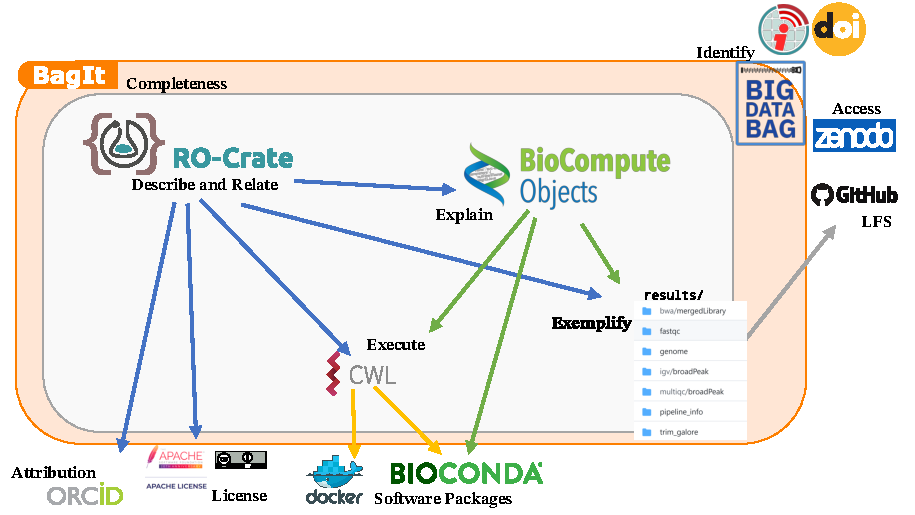
\includegraphics[width=\textwidth]{figures/ch05/ro-crate-bco-sep-of-concerns.pdf}
	\caption[Separation of Concerns in BCO RO-Crate]{\textbf{Separation of Concerns in BCO RO-Crate}. BioCompute
  Object (IEEE2791) is a JSON file that structurally explains the purpose
  and implementation of a computational workflow, for instance
  implemented in Common Workflow Language (CWL), that installs the
  workflow's software dependencies as Docker containers or BioConda
  packages. An example execution of the workflow shows the different
  kinds of result outputs, which may be external, using GitHub LFS \cite {GitHub 2021} to support larger data. RO-Crate gathers all these local
  and external resources, relating them and giving individual
  descriptions, for instance permanent DOI identifiers for reused
  datasets accessed from Zenodo, but also adding external identifiers to
  attribute authors using ORCID or to identify which licences apply to
  individual resources. The RO-Crate and its local files are captured in
  a BagIt whose checksum ensures completeness, combined with Big Data Bag
  \cite{Chard 2016} features to ``complete'' the
  bag with large external files such as the workflow outputs.}
  \label{ch5:fig:sep_concerns}
\end{figure}


\hypertarget{culturalheritage}{%
\subsubsection{Digital Humanities: Cultural
Heritage}\label{ch5:culturalheritage}}

The Pacific And Regional Archive for Digital Sources in Endangered
Cultures (PARADISEC\footnote{\url{https://www.paradisec.org.au/}}) \cite{Thieberger 2012}
maintains a repository of more than 500,000 files documenting
endangered languages across more than 16,000 items, collected and
digitised over many years by researchers interviewing and recording
native speakers across the region.

The Modern PARADISEC demonstrator\footnote{\url{https://mod.paradisec.org.au/}} has
been
proposed\footnote{\url{https://arkisto-platform.github.io/case-studies/paradisec/}}
as an update to the 18 year old infrastructure, to also help long-term
preservation of these artefacts in their digital form. The demonstrator
uses RO-Crate to describe the overall structure and to capture the
metadata of each item. The existing PARADISEC data collection has been
ported and captured as RO-Crates. A Web portal then exposes the
repository and its entries by indexing the RO-Crate metadata files,
presenting a domain-specific view of the items -- the RO-Crate is
``hidden'' and does not change the user interface.


The PARADISEC use case takes advantage of several RO-Crate features and
principles. Firstly, the transcribed metadata are now independent of the
PARADISEC platform and can be archived, preserved and processed in its
own right, using schema.org as base vocabulary and extended with
PARADISEC-specific terms.

In this approach, RO-Crate is the holder of itemised metadata, stored in
regular files that are organised using
Oxford Common File
Layout\footnote{\url{https://ocfl.io/1.0/spec/}} (OCFL)
\cite{OCFL 2020}, which ensures file integrity
and versioning on a regular shared file system. This lightweight
infrastructure also gives flexibility for future developments and
maintenance. For example a consumer can use Linked Data software such as
a graph database and query the whole corpora using SPARQL triple
patterns across multiple RO-Crates. For long term digital preservation,
beyond the lifetime of PARADISEC portals, a ``last resort'' fallback is
storing the generic RO-Crate HTML preview
\cite{ro-crate-html-js}. Such
human-readable rendering of RO-Crates can be hosted as static files by
any Web server, in line with the approach taken by the Endings
Project.\footnote{The Endings Project \url{https://endings.uvic.ca/} 
  is a five-year project funded by the Social Sciences and Humanities
  Research Council (SSHRC) that is creating tools, principles, policies
  and recommendations for digital scholarship practitioners to create
  accessible, stable, long-lasting resources in the humanities.}

\subsubsection{Machine-actionable Data Management Plans}\label{ch5:dmp}

Machine-actionable Data Management Plans (maDMPs) have been proposed as
an improvement to automate FAIR data management tasks in research
\cite{Miksa 2019b}; maDMPs
use PIDs and controlled vocabularies to describe what happens to data
over the research life cycle
\cite{Cardoso 2020a}. The
Research Data Alliance's \emph{DMP Common Standard} for maDMPs
\cite{Miksa 2019a} is one such
formalisation for expressing maDMPs, which can be expressed as Linked
Data using the DMP Common Standard Ontology
\cite{Cardoso 2020b}, a
specialisation of the W3C Data Catalog Vocabulary (DCAT)
\cite{Albertoni 2020}.
RDA maDMPs are usually expressed using regular JSON, conforming to the
DMP JSON Schema.

A mapping has been produced between Research Object Crates and
Machine-actionable Data Management Plans
\cite{Miksa 2020}, implemented by
the RO-Crate RDA maDMP Mapper
\cite{Arfaoui 2020}. A similar
mapping has been implemented by \emph{RO-Crate\_2\_ma-DMP}
\cite{Brenner 2020}. In both cases,
a maDMP can be converted to a RO-Crate, or vice versa. In
\cite{Miksa 2020} this
functionality caters for two use cases:

\begin{enumerate}
\item
  Start a skeleton data management plan based on an existing RO-Crate
  dataset, e.g.~an RO-Crate from WorkflowHub.
\item
  Instantiate an RO-Crate based on a data management plan.
\end{enumerate}

An important nuance here is that data management plans are (ideally)
written in \emph{advance} of data production, while RO-Crates are
typically created to describe data \emph{after} it has been generated.
What is significant to note in this approach is the importance of
\textbf{templating} in order to make both tasks automatable and
achievable, and how RO-Crate can fit into earlier stages of the research
life cycle.

\subsubsection{Institutional data repositories -- Harvard Data Commons}
\label{ch5:institutionalrepos}

The concept of a \textbf{Data Commons} for research collaboration was
originally defined as \emph{``cyber-infrastructure that co-locates data,
storage, and computing infrastructure with commonly used tools for
analysing and sharing data to create an interoperable resource for the
research community''}
\cite{Grossman 2016}. More recently,
Data Commons has been established to mean integration of active
data-intensive research with data management and archival best
practices, along with a supporting computational infrastructure.
Furthermore, the Commons features tools and services, such as
computation clusters and storage for scalability, data repositories for
disseminating and preserving regular, but also large or sensitive
datasets, and other research assets. Multiple initiatives were
undertaken to create Data Commons on national, research, and
institutional levels. For example, the Australian Research Data Commons
(ARDC)\footnote{\url{https://ardc.edu.au/}} 
\cite{Barker 2019} is a national
initiative that enables local researchers and industries to access
computing infrastructure, training, and curated datasets for
data-intensive research. NCI's Genomic
Data Commons\footnote{\url{https://gdc.cancer.gov/}} (GDC)
\cite{Jensen 2017} provides
the cancer research community with access to a vast volume of genomic
and clinical data. Initiatives such as
Research Data Alliance (RDA) Global Open Research Commons\footnote{\url{https://www.rd-alliance.org/groups/global-open-research-commons-ig}}
propose standards for
the implementation of Data Commons to prevent them becoming ``data
silos'' and thus, enable interoperability from one Data Commons to
another.

\textbf{Harvard Data Commons}
\cite{Crosas 2020} aims to address the
challenges of data access and cross-disciplinary research within a
research institution. It brings together multiple institutional schools,
libraries, computing centres and the
Harvard
Dataverse\footnote{\url{https://dataverse.harvard.edu/}} data repository.
Dataverse\footnote{\url{https://dataverse.org/}}
\cite{Crosas 2011} is a free
and open-source software platform to archive, share and cite research
data. The Harvard Dataverse repository is the largest of 70 Dataverse
installations worldwide, containing over 120K datasets with about 1.3M
data files (as of 2021-11-16). Working toward the goal of facilitating
collaboration and data discoverability and management within the
university, Harvard Data Commons has the following primary objectives:

\begin{enumerate}
\item
  The integration of Harvard Research Computing with Harvard Dataverse
  by leveraging Globus endpoints
  \cite{Chard 2014}; this will allow
  an automatic transfer of large datasets to the repository. In some
  cases, only the metadata will be transferred while the data stays
  stored in remote storage.
\item
  Support for advanced research workflows and providing packaging
  options for assets such as code and workflows in the Harvard Dataverse
  repository to enable reproducibility and reuse.
\item
  Interation of repositories supported by Harvard, which include
  DASH\footnote{\url{https://dash.harvard.edu/}}, the open access institutional
  repository, the Digital Repository Services (DRS) for preserving
  digital asset collections, and the Harvard Dataverse.
\end{enumerate}

Particularly relevant to this article is the second objective of the
Harvard Data Commons, which aims to support the deposit of research
artefacts to Harvard Dataverse with sufficient information in the
metadata to allow their future reuse (Figure \vref{ch5:fig:hdc}). To support the incorporation of data, code, and other artefacts
from various institutional infrastructures, Harvard Data Commons is
currently working on RO-Crate adaptation. The RO-Crate metadata provides
the necessary structure to make all research artefacts FAIR. The
Dataverse software already has
extensive
support\footnote{\url{https://guides.dataverse.org/en/latest/user/appendix.html}} for metadata, including the Data Documentation Initiative
(DDI), Dublin Core, DataCite, and schema.org. Incorporating RO-Crate,
which has the flexibility to describe a wide range of research
resources, will facilitate their seamless transition from one
infrastructure to the other within the Harvard Data Commons.

Even though the Harvard Data Commons is specific to Harvard University,
the overall vision and the three objectives can be abstracted and
applied to other universities or research organisations. The Commons
will be designed and implemented using standards and commonly-used
approaches to make it interoperable and reusable by others.

\begin{figure}%[t!]
  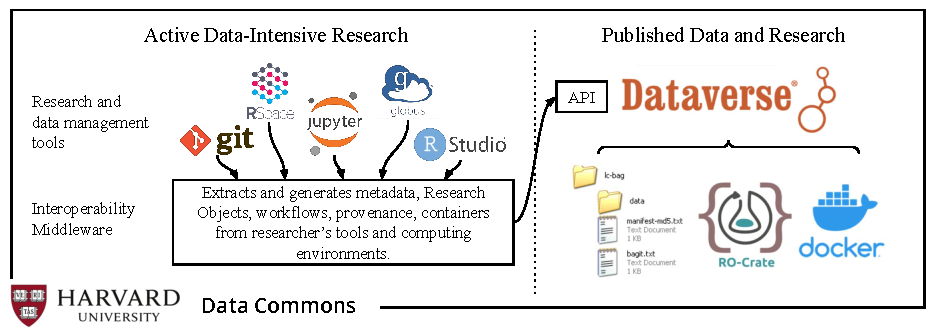
\includegraphics[width=1.1\textwidth]{figures/ch05/data-commons-ro-crate-figure-5.pdf}
	\caption[Harvard Data Commons]{\textbf{One aspect of Harvard Data Commons}. Automatic
  encapsulation and deposit of artefacts from data management tools used
  during active research at the Harvard Dataverse repository.}
  \label{ch5:fig:hdc}
\end{figure}

\subsection{Related Work}\label{ch5:relatedwork}

With the increasing digitisation of research processes, there has been a
significant call for the wider adoption of interoperable sharing of data
and its associated metadata. We refer to
\cite{Koesten 2020} for a
comprehensive overview and recommendations, in particular for data;
notably that review highlights the wide variety of metadata and
documentation that the literature prescribes for enabling data reuse.
Likewise, we suggest
\cite{Leipzig 2021} that
covers the importance of metadata standards in reproducible
computational research.

Here we focus on approaches for bundling research artefacts along with
their metadata. This notion of publishing compound objects for scholarly
communication has a long history behind it
\cite{Claerbout 1992,Van de Sompel 2007},
but recent approaches have followed three main strands: (i) publishing to
centralised repositories; (ii) packaging approaches similar to RO-Crate;
and (iii) bundling the computational workflow around a scientific
experiment.

\subsubsection{Bundling and Packaging Digital Research
Artefacts}\label{ch5:bundling-and-packaging-digital-research-artefacts}

Early work making the case for publishing compound scholarly
communication units
\cite{Van de Sompel 2007}
led to the development of the
Object Re-Use and Exchange
model\footnote{\url{http://www.openarchives.org/ore/1.0/primer}} (OAI-ORE), providing a structured \textbf{resource map}
of the digital artefacts that together support a scholarly output.

The challenge of describing computational workflows was one of the main
motivations for the early proposal of \emph{Research Objects} (RO)
\cite{Bechhofer 2013}
as first-class citizens for sharing and publishing. The RO approach
involves bundling datasets, workflows, scripts and results along with
traditional dissemination materials like journal articles and
presentations, forming a single package. Crucially, these resources are
not just gathered, but also individually typed, described and related to
each other using semantic vocabularies. As pointed out in
\cite{Bechhofer 2013} an
open-ended \emph{Linked Data} approach is not sufficient for scholarly
communication: a common data model is also needed in addition to common
and best practices for managing and annotating lifecycle, ownership,
versioning and attributions.

Considering the FAIR principles
\cite{Wilkinson 2016}, we can say with
hindsight that the initial RO approaches strongly targeted
\emph{Interoperability}, with a particular focus on the reproducibility
of \emph{in-silico experiments} involving computational workflows and
the reuse of existing RDF vocabularies.

The first implementation of Research Objects for sharing workflows in
myExperiment \cite{Goble 2010} was
based on RDF ontologies
\cite{Newman 2009}, building on
Dublin Core, FOAF, SIOC, Creative Commons and OAI-ORE to form
myExperiment ontologies for describing social networking, attribution
and credit, annotations, aggregation packs, experiments, view
statistics, contributions, and workflow components
\cite{myExperiment 2009}.

This initially workflow-centric approach was further formalised as the
Wf4Ever Research Object Model
\cite{Belhajjame 2015}, which is
a general-purpose research artefact description framework. This model is
based on existing ontologies (FOAF, Dublin Core Terms, OAI-ORE and
AO/OAC precursors to the W3C Web Annotation Model
\cite{Ciccarese 2017})
and adds specializations for workflow models and executions using W3C
PROV-O \cite{Lebo 2013a}.
The Research Object statements are saved in a \emph{manifest} (the
OAI-ORE \emph{resource map}), with additional annotation resources
containing user-provided details such as title and description.

We now claim that one barrier for wider adoption of the Wf4Eer Research
Object model for general packaging digital research artefacts was
exactly this re-use of multiple existing vocabularies (FAIR principle
I2: \emph{Metadata use vocabularies that follow FAIR principles}), which
in itself is recognised as a challenge
\cite{Katsumi 2016}. Adapters
of the Wf4Ever RO model would have to navigate documentation of multiple
overlapping ontologies, in addition to facing the usual Semantic Web
development choices for RDF serialization formats, identifier minting
and publishing resources on the Web.

Several developments for Research Objects improved on this situation,
such as ROHub used by Earth Sciences
\cite{Garcia-Silva 2019}, which provides a
user-interface for making Research Objects, along with Research Object
Bundle \cite{Soiland-Reyes 2014} (RO
Bundle), which is a ZIP-archive embedding data files and a JSON-LD
serialization of the manifest with mappings for a limited set of terms.
RO Bundle was also used for storing detailed workflow run provenance
(TavernaPROV
\cite{Soiland-Reyes 2016}).

RO-Bundle evolved to Research Object
BagIt archives\footnote{\url{https://w3id.org/ro/bagit}}, a variant of RO Bundle as a BagIt archive
\cite{Kunze 2018}, used by Big Data Bags
\cite{Chard 2016},
CWLProv \cite{Khan 2019} and
WholeTale \cite{Chard 2020,Chard 2019}.

\subsubsection{FAIR Digital Objects}\label{ch5:fair-digital-objects}

FAIR Digital Objects (FDO)
\cite{De Smedt 2020} have been
proposed as a conceptual framework for making digital resources
available in a Digital Objects (DO) architecture which encourages active
use of the objects and their metadata. In particular, an FDO has five
parts: (i) The FDO \emph{content}, bit sequences stored in an accessible
repository; (ii) a \emph{Persistent Identifier} (PID) such as a DOI that
identifies the FDO and can resolve these same parts; (iii) Associated
rich \emph{metadata}, as separate FDOs; (iv) Type definitions, also
separate FDOs; (v) Associated \emph{operations} for the given types. A
Digital Object typed as a Collection aggregates other DOs by reference.

The Digital Object Interface Protocol \cite{DONA 2018}
can be considered an ``abstract protocol'' of requirements, DOs could be
implemented in multiple ways. One suggested implementation is the 
FAIR Digital Object
Framework,\footnote{\url{https://fairdigitalobjectframework.org/}} based on HTTP and the Linked Data Principles. While there is
agreement on using PIDs based on DOIs, consensus on how to represent
common metadata, core types and collections as FDOs has not yet been
reached. We argue that RO-Crate can play an important role for FDOs:

\begin{enumerate}
\item
  By providing a predictable and extensible serialisation of structured
  metadata.
\item
  By formalising how to aggregate digital objects as collections (and
  adding their context).
\item
  By providing a natural Metadata FDO in the form of the RO-Crate
  Metadata File.
\item
  By being based on Linked Data and schema.org vocabulary, meaning that
  PIDs already exist for common types and properties.
\end{enumerate}

At the same time, it is clear that the goal of FDO is broader than that
of RO-Crate; namely, FDOs are active objects with distributed
operations, and add further constraints such as PIDs for every element.
These features improve FAIR features of digital objects and are also
useful for RO-Crate, but they also severely restrict the infrastructure
that needs to be implemented and maintained in order for FDOs to remain
accessible. RO-Crate, on the other hand, is more flexible: it can
minimally be used within any file system structure, or ideally exposed
through a range of Web-based scenarios. A \emph{FAIR profile of
RO-Crate} (e.g.~enforcing PID usage) will fit well within a FAIR Digital
Object ecosystem.

\subsubsection{Packaging Workflows}\label{ch5:packaging-workflows}

The use of computational workflows, typically combining a chain of tools
in an analytical pipeline, has gained prominence in particular in the
life sciences. Workflows might be used primarily to improve
computational scalability, as well as to assist in making computed data
results FAIR \cite{Goble 2020}, for
instance by improving reproducibility
\cite{Cohen-Boulakia 2017}, but also
because programmatic data usage help propagate their metadata and
provenance \cite{Kim 2008}. At the
same time, workflows raise additional FAIR challenges, since they can be
considered important research artefacts themselves. This viewpoint poses
the problem of capturing and explaining the computational methods of a
pipeline in sufficient machine-readable detail
\cite{Lamprecht 2019}.

Even when researchers follow current best practices for workflow
reproducibility
\cite{Grüning 2018b,Cohen-Boulakia 2017}, the
communication of computational outcomes through traditional academic
publishing routes effectively adds barriers as authors are forced to
rely on a textual manuscript representations. This hinder
reproducibility and FAIR use of the knowledge previously captured in the
workflow.

As a real-life example, let us look at a metagenomics article
\cite{Almeida 2019} that describes
a computational pipeline. Here the authors have gone to extraordinary
efforts to document the individual tools that have been reused,
including their citations, versions, settings, parameters and
combinations. The \emph{Methods} section is two pages in tight
double-columns with twenty four additional references, supported by the
availability of data on an FTP server (60 GB)
\cite{EMBL-EBI 2019}
and of open source code in GitHub
Finn-Lab/MGS-gut\footnote{\url{https://github.com/Finn-Lab/MGS-gut}}
\cite{EMBL-EBI 2020}, including the
pipeline as shell scripts and associated analysis scripts in R and
Python.

This attention to reporting detail for computational workflows is
unfortunately not yet the norm, and although bioinformatics journals
have strong \emph{data availability} requirements, they frequently do
not require authors to include or cite \emph{software, scripts and
pipelines} used for analysing and producing results \cite{Soiland-Reyes 2020a}.
Indeed, in the absence of a specific requirement and an editorial policy
to back it up -- such as eliminating the reference limit -- authors are
effectively discouraged from properly and comprehensively citing
software \cite{Nature 2019}.

However detailed this additional information might be, another
researcher who wants to reuse a particular computational method may
first want to assess if the described tool or workflow is Re-runnable
(executable at all), Repeatable (same results for original inputs on
same platform), Reproducible (same results for original inputs with
different platform or newer tools) and ultimately Reusable (similar
results for different input data), Repurposable (reusing parts of the
method for making a new method) or Replicable (rewriting the workflow
following the method description)
\cite{Benureau 2017,Goble 2016}.

Following the textual description alone, researchers would be forced to
jump straight to evaluate ``Replicable'' by rewriting the pipeline from
scratch. This can be expensive and error-prone. They would firstly need
to install all the software dependencies and download reference
datasets. This can be a daunting task, which may have to be repeated
multiple times as workflows typically are developed at small scale on
desktop computers, scaled up to local clusters, and potentially put into
production using cloud instances, each of which will have different
requirements for software installations.

In recent years the situation has been greatly improved by software
packaging and container technologies like Docker and Conda, these
technologies have been increasingly adopted in life sciences
\cite{Möller 2017} thanks to
collaborative efforts such as BioConda
\cite{Grüning 2018a} and
BioContainers
\cite{da Veiga Leprevost 2017}, and
support by Linux distributions (e.g.~Debian Med
\cite{Möller 2010}). As of
November 2021, more than 9,000 software packages are available in
BioConda alone,\footnote{\url{https://anaconda.org/bioconda/}} and 10,000 containers
in BioContainers.\footnote{\url{https://biocontainers.pro/\#/registry}}

Docker and Conda have been integrated into workflow systems such as
Snakemake
\cite{Köster 2012}, Galaxy
\cite{Afgan 2018} and Nextflow
\cite{Di Tommaso 2017}, meaning
a downloaded workflow definition can now be executed on a ``blank''
machine (except for the workflow engine) with the underlying analytical
tools installed on demand. Even with using containers there is a
reproducibility challenge, for instance Docker Hub's retention policy
will expire container images after six
months,\footnote{\url{https://www.docker.com/blog/docker-hub-image-retention-policy-delayed-and-subscription-updates/}}
or a lack of recording versions of transitive dependencies of Conda
packages could cause incompatibilities if the packages are subsequently updated.

These container and package systems only capture small amounts of
metadata\footnote{Docker and Conda can use \emph{build recipes}, a set
  of commands that construct the container image through downloading and
  installing its requirements. However these recipes are effectively
  another piece of software code, which may itself decay and become
  difficult to rerun.}. In particular, they do not capture any of the
semantic relationships between their content. Understanding these
relationships is made harder by the opaque wrapping of arbitrary tools
with unclear functionality, licenses and attributions.

From this we see that computational workflows are themselves complex
digital objects that need to be recorded not just as files, but in the
context of their execution environment, dependencies and analytical
purpose in research -- as well as other metadata (e.g.~version, license,
attribution and identifiers).

It is important to note that having all these computational details in
order to represent them in an RO-Crate is an ideal scenario -- in
practice there will always be gaps of knowledge, and exposing all
provenance details automatically would require improvements to the data
sources, workflow, workflow engine and its dependencies. RO-Crate can be
seen as a flexible annotation mechanism for augmenting automatic
workflow provenance. Additional metadata can be added manually, e.g.~for
sensitive clinical data that cannot be publicly exposed\footnote{FAIR
  principle A2: \emph{Metadata are accessible, even when the data are no
  longer available.}
  \cite{Wilkinson 2016}}, or to cite
software that lack persistent identifiers. This inline \emph{FAIRifying}
allows researchers to achieve ``just enough FAIR'' to explain their
computational experiments.

\hypertarget{conclusion}{%
\subsection{Conclusion}\label{ch5:conclusion}}

RO-Crate has been established as an approach to packaging digital
research artefacts with structured metadata. This approach assists
developers and researchers to produce and consume FAIR archives of their
research.

RO-Crate is formed by a set of best practice recommendations, developed
by an open and broad community. These guidelines show how to use ``just
enough'' standards in a consistent way. The use of structured metadata
with a rich base vocabulary can cover general-purpose contextual
relations, with a Linked Data foundation that ensures extensibility to
domain- and application-specific uses. We can therefore consider an
RO-Crate not just as a structured data archive, but as a multimodal
scholarly knowledge graph that can help ``FAIRify'' and combine metadata
of existing resources.

The adoption of simple Web technologies in the RO-Crate specification
has helped a rapid development of a wide variety of supporting open
source tools and libraries. RO-Crate fits into the larger landscape of
open scholarly communication and FAIR Digital Object infrastructure, and
can be integrated into data repository platforms. RO-Crate can be
applied as a data/metadata exchange mechanism, assist in long-term
archival preservation of metadata and data, or simply used at a small
scale by individual researchers. Thanks to its strong community support,
new and improved profiles and tools are being continuously added to the
RO-Crate landscape, making it easier for adopters to find examples and
support for their own use case.

\subsubsection{Strictness vs
flexibility}\label{ch5:strictness-vs-flexibility}

There is always a tradeoff between flexibility and strictness \cite{Troncy 2010}
when deciding on semantics of metadata models. Strict requirements make
it easier for users and code to consume and populate a model, by
reducing choices and having mandated ``slots'' to fill in. But such
rigidity can also restrict richness and applicability of the model, as
it in turn enforce the initial assumptions about what can be described.

RO-Crate attempts to strike a balance between these tensions, and
provides a common metadata framework that encourages extensions.
However, just like the RO-Crate specification can be thought of as a
\emph{core profile} of schema.org in JSON-LD, we cannot stress the
importance of also establishing domain-specific RO-Crate profiles and
conventions, as explored in Sections~\vref{ch5:profiles} and \vref
{ch5:inuse}. Specialization comes
hand-in-hand with the principle of \emph{graceful degradation}; RO-Crate
applications and users are free to choose the semantic detail level they
participate at, as long as they follow the common syntactic
requirements.

\subsection{Future Work}\label{ch5:futurework}

The direction of future RO-Crate work is determined by the community
around it as a collaborative effort. We currently plan on further
outreach, building training material (including a comprehensive
entry-level tutorial) and maturing the reference implementation
libraries. We will also collect and build examples of RO-Crate
\emph{consumption}, e.g.~Jupyter Notebooks that query multiple crates
using knowledge graphs. In addition, we are exploring ways to support
some entity types requested by users, e.g.~detailed workflow runs or
container provenance, which do not have a good match in schema.org. Such
support could be added, for instance, by integrating other vocabularies
or by having separated (but linked) metadata files.

Furthermore, we want to better understand how the community uses
RO-Crate in practice and how it contrasts with other related efforts;
this will help us to improve our specification and tools. By discovering
commonalities in emerging usage (e.g.~additional schema.org types), the
community helps to reduce divergence that could otherwise occur with
proliferation of further RO-Crate profiles. We plan to gather feedback
via user studies, with the Linked Open Data community or as part of EOSC
Bring-your-own-Data training events.

We operate in an open community where future and potential users of
RO-Crate are actively welcomed to participate and contribute feedback
and requirements. In addition, we are targeting a wider audience through
extensive
outreach
activities\footnote{\url{https://www.researchobject.org/ro-crate/outreach.html}} and by initiating new connections. Recent contacts include
American Geophysical Union (AGU) on Data Citation Reliquary
\cite{Agarwal 2021}, National
Institute of Standards and Technology (NIST) on material science, and
InvenioRDM\footnote{\url{https://inveniosoftware.org/products/rdm/}} used by the
Zenodo data repository. New Horizon Europe projects adapting RO-Crate
include BY-COVID,\footnote{\url{https://by-covid.org/}} which aims to improve FAIR
access to data on COVID-19 and other infectious diseases.

The main addition in the upcoming 1.2 release of the RO-Crate
specifications will be the formalization of
profiles\footnote{\url{https://www.researchobject.org/ro-crate/1.2-DRAFT/profiles}}
for different categories of crates. Additional entity types have been
requested by users, e.g. workflow runs, business workflows, containers
and software packages, tabular data structures; these are not always
matched well with existing schema.org types, but may benefit from other
vocabularies or even separate metadata files, e.g. from Frictionless
Data.\footnote{\url{https://frictionlessdata.io/}} We will be further aligning
and collaborating with related research artefact description efforts
like CodeMeta\footnote{\url{https://codemeta.github.io/}} for software metadata,
Science-on-Schema.org\footnote{\url{https://science-on-schema.org/}}
\cite{Jones 2021} for datasets, FAIR Digital
Objects\footnote{\url{https://fairdo.org/}} \cite{De Smedt 2020} and
activities in EOSC task forces\footnote{\url{https://www.eosc.eu/task-force-faq}}
including the EOSC Interoperability Framework \cite{Kurowski 2021}.
